
\section{Work and Kinetic Energy\footnote{
1990-93 Dept. of Physics and Astronomy, Dickinson College. Supported by FIPSE
(U.S. Dept. of Ed.) and NSF. Portions of this material have been modified locally
and may not have been classroom tested at Dickinson College.
}}

\makelabheader %(Space for student name, etc., defined in master.tex or labmanual_formatting_commands.tex)

\bigskip
\textbf{Objectives} 

\begin{itemize}[nosep]
\item To discover Hooke's law. 
\item To understand the concept of kinetic energy and its relationship to work as
embodied in the work-energy theorem. 
\item To develop an understanding of the physical significance of mathematical integration.
\end{itemize}

\bigskip
\textbf{The Force Exerted on a Mass by an Extended Spring} 

So far we have pushed and pulled on an object with a constant force and calculated
the work needed to displace that object. In most real situations the force on
an object can change as it moves. 

What happens to the average force needed to stretch a spring from 0 to 1 cm
compared to the average force needed to extend the same spring from 10 to 11
cm? How does the applied force on a spring affect the amount by which it stretches,
i.e., its displacement?

\bigskip

\textbf{Apparatus }

\begin{itemize}[nosep]
\item A large spring 
\item A support rod to hang the spring 
\item A 2-meter stick 
\item A variety of masses
\end{itemize}
\textbf{Activity 1: Are Spring Forces Constant?} 

Hang the spring from a support rod with the large diameter coils in the downward
position. Extend the spring from 0 to 1 cm. Feel the force needed to extend
the spring. Extend the spring from 10 to 11 cm. Feel the force needed to extend
the spring again. How do the two forces compare? Are they the same? 
\vspace{10mm}

\textbf{The Force and Work Needed to Stretch a Spring} 

Now we would like to be able to quantify the force and work needed to extend
a spring as a function of its displacement from an equilibrium position (i.e.,
when it is ``unstretched'').

\textbf{Activity 2: Force \textit{vs.}~Displacement for a Spring }

(a) Measure the distance from the floor to the lower end of the spring and record this distance as \( s_{0} \) below. 
Start filling in the first four columns of the data table on the next page.
(Alternatively, this data table can be created directly in \textit{Excel}. 
If you use \textit{Excel}, print the data table and attach it to this lab.)
Hang different masses on the spring in 0.100~kg increments up to 1.000~kg and calculate the external gravitational force  $F_{\rm ext}$ applied to the spring.  
For each mass, measure the distance $s$ from the floor to the lower end of the spring, and also calculate the stretch of the spring $x ~(= s_0 - s)$.  

\hspace{0.5in}$s_0 =$
\bigskip

\begin{center}
{\renewcommand{\arraystretch}{1.8}
\begin{tabular}{|c|c|C{0.5in}|C{0.5in}|c|c|c|c|} \hline 
$m$ (kg) & $s$ (m) & $x$ (m) &
$\Delta  x$ (m) &  $F_{\rm ext}$ (N) & $\langle F_{\rm ext} \rangle$ (N) & $\Delta  W$ (J) & $W_{\rm total}$ (J) \\
\hhline{|=|=|=|=|=|=|=|=|}
0.0 & & 0.0 & - & 0.0 & - & - & 0.0 \\ \hline 
0.1 & & & & & & & \\ \hline 
0.2 & & & & & & & \\ \hline 
0.3 & & & & & & & \\ \hline 
0.4 & & & & & & & \\ \hline 
0.5 & & & & & & & \\ \hline
0.6 & & & & & & & \\ \hline 
0.7 & & & & & & & \\ \hline 
0.8 & & & & & & & \\ \hline 
0.9 & & & & & & & \\ \hline 
1.0 & & & & & & & \\ \hline 
\end{tabular} }
\end{center}



(b) Using \textit{Excel}, create a graph of \( F_{\rm ext} \) (vertical axis) \textit{vs.}~$x$ (horizontal axis). Is the graph linear?
If the force, \( F_{\rm ext} \), increases with the displacement in a proportional
way, fit the data with a linear function including a trendline with equation. 
Print the graph and include a copy with this unit. Use the LINEST function 
in \textit{Excel} (see \textbf{Appendix \ref{excel}: Excel}) to determine the slope of the 
line and its uncertainty. Use the symbol $k$ to represent the slope of the line.
Record your value of $k$ and its uncertainty here. What are its units? 
Note:  $k$ is known as the spring constant.
\answerspace{15mm}

(c) Write the equation describing the relationship between the external force,
\( F_{\rm ext} \), and the total displacement, 
$x$, of the spring from its equilibrium
using the symbols \( F_{\rm ext} \), $k$, and $x$.
\answerspace{15mm}

Note: Any restoring force on an object which is proportional to its displacement
is known as a Hooke's Law Force. There was an erratic, contentious genius named
Robert Hooke who was born in 1635. He played with springs and argued with 
Newton.

\bigskip
\textbf{Calculating Work when the Force is not Constant }

We would like to expand the definition of work so it can be used to calculate
the work associated with stretching a spring and the work associated with other
forces that are not constant. A helpful approach is to plot the average force
needed to move an object for each successive displacement \( \Delta  x\) as
a bar graph like that shown in the figure below. The figure shows a graph representing
the average applied force causing each unit of displacement of an object. This
graph represents force that is not constant but not the force \textit{vs.}~displacement
of a typical spring.

Note: The bar graph below is intended to illustrate mathematical concepts. Any
similarity between the values of the forces in the bar graph and any real set
of forces is purely coincidental. In general, the force causing work to be done
on an object is not constant.

\vspace{0.3cm}
%{\par\centering 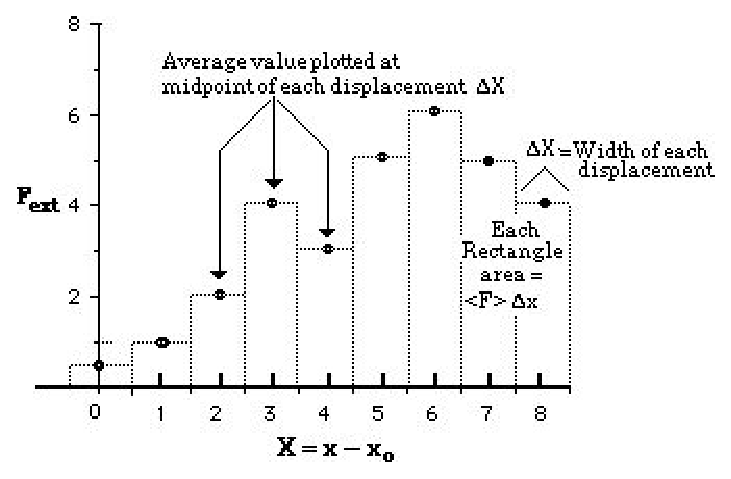
\includegraphics{work_kinetic/work_kinetic_fig1.eps} \par}
{\par\centering 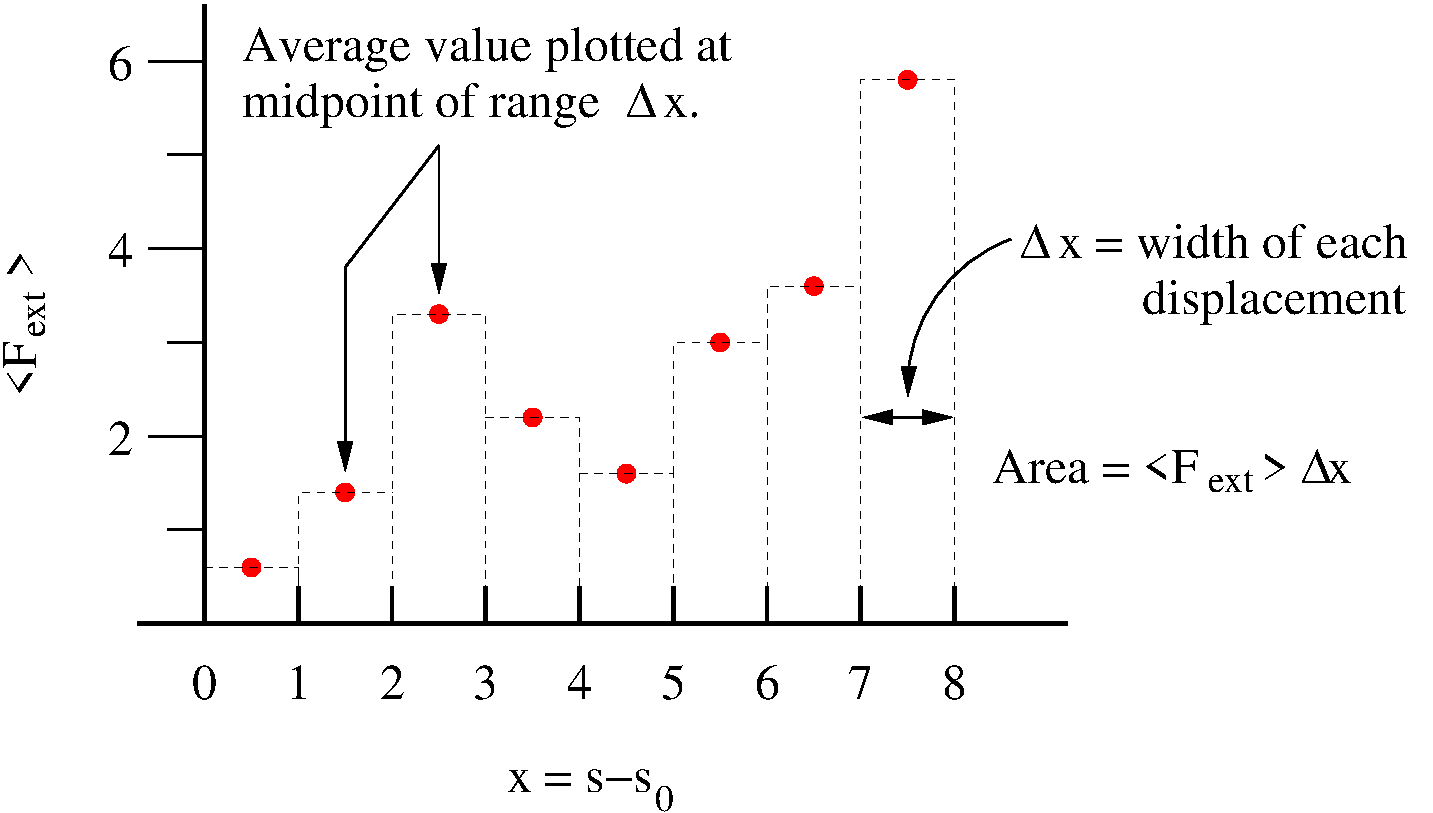
\includegraphics[height=2.75in]{work_kinetic/workAndKEF1.pdf} \par}
\index{color page}
\vspace{0.3cm}

\textbf{Activity 3: Force \textit{vs.}~Distance in a Bar Graph }

(a) Using your data from Activity 2, calculate the width of each displacement, \( \Delta x \), and the average external force, \(\langle F_{\rm ext} \rangle\) for each displacement, and record the values in the table above. This means for each mass take an average of the force value and the previous force value. You now have columns 5 and 6 filled in. Plot \( \langle F_{\rm ext} \rangle\) \textit{vs.}~$x$ as a bar graph on the grid below.  (Choose appropriate scales for the axes before making the graph.) Alternatively, you can plot the bar graph in \textit{Excel}.

%\vspace{0.3cm}
%{\par\centering 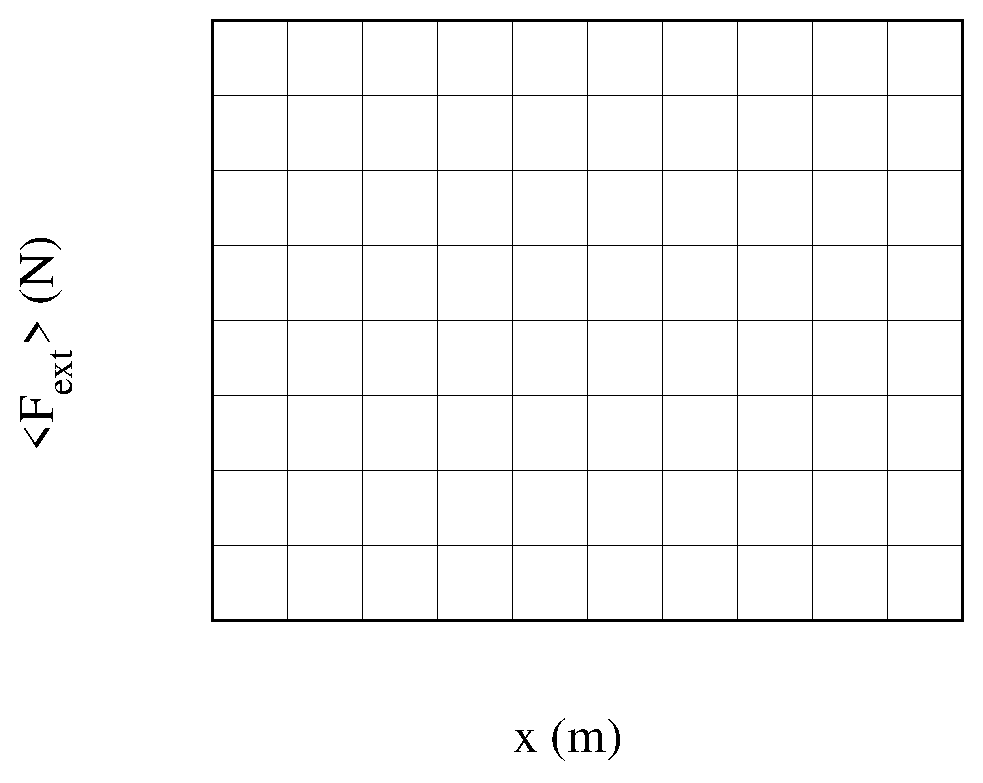
\includegraphics[height=3.250in]{work_kinetic/workAndKEF2.eps} \par}
%\vspace{0.3cm}
\begin{lab_axis}*[lab_grid,
	height = 2.7in, width = 4.5in,
	xlabel={Position $x$ (m)},
	ylabel={Average force $\langle F_{\rm ext} \rangle$ (N)},
	xmin=0, xmax=10,
	ymin=0, ymax=6,
	xtick distance = 12,  %tricking it into ONLY putting a tick label at x=0, y=0
	ytick distance = 7,
	minor y tick num=6,
	minor x tick num=11,
	]
\end{lab_axis}

How can we calculate the work done in stretching the spring? We can use several
equivalent techniques: (1)~adding up little pieces of \( \langle F_{\rm ext} 
\rangle \Delta x \) from the above bar graph,
(2)~finding the area under the ``curve'' you created in Activity 2, or 
(3)~using mathematical integration.

All three methods should yield about the same result. If you have not yet encountered
integrals in a calculus course, you can compare the results of using the first
two methods. If you have studied integrals in calculus you may want to consult
your instructor or the textbook about how to set up the appropriate definite
integral to calculate the work needed to stretch the spring. 

\pagebreak[3]
\textbf{Activity 4: Calculation of Work }

(a) Calculate the work needed to stretch the spring by calculating small increments of \( \langle F_{\rm ext} \rangle \Delta  x\) (this is \( \Delta W\), or column 7 in your table). Record the running sum in the table (this is \( W_{\rm total} \), or column 8) for each mass. (The ``running sum'' is the sum of all the values of \( \Delta W\) up to that point.) Indicate the final value of \( W_{\rm total} \) below. Don't forget to specify units.
\vspace{5mm}

\( W_{\rm total} =\) 
\vspace{5mm}

(b) Calculate the work needed to stretch the spring by computing the area under
the curve in the graph of \( F_{\rm ext} \) \textit{vs.}~$x$ that you created in Activity 2.
\answerspace{20mm}

(c) Calculate the work needed to stretch the spring by computing the definite 
integral of the function you found in Activity 2(c), evaluated from the 
initial $x$ value to the final $x$ value.
\answerspace{20mm}

(d) Do the three values of the work done agree with one another? How would 
you account for any discrepancy?
\answerspace{20mm}


\textbf{Defining Kinetic Energy and Its Relationship to Work} 

What happens when you apply an external force to an object that is free to move
and has no friction forces on it? Obviously it should experience an acceleration
and end up being in a different state of motion. Can we relate the change in
motion of the object to the amount of work that is done on it?

Let's consider a fairly simple situation. Suppose an object is lifted through
a distance $s$ near the surface of the earth and then allowed to fall. During
the time it is falling it will experience a constant force as a result of the
attraction between the object and the earth glibly called the force of gravity.
You can use the theory we have already developed for the gravitational force
to compare the velocity of the object to the work done on it by the gravitational
field as it falls through a distance 
$y$. This should lead naturally to the definition
of a new quantity called kinetic energy, which is a measure of the amount of
``motion'' gained as a result of the work done on the mass. 

\textbf{Activity 5: Equations for Falling $v$ \textit{vs.}~$y$ }

(a) An object of mass m is dropped near the surface of the earth. What are the
magnitude and direction of its acceleration $g$?
\answerspace{10mm}

(b) If the object has no initial velocity and is allowed to fall for a time
$t$ under the influence of the gravitational force, what kinematic equation describes the relationship between the distance the object falls, $y$, and its time of fall, $t$? Assume \( y_{0}=0 \) and take positive down.
\answerspace{10mm}

\pagebreak[2]
(c) Do you expect the magnitude of the velocity to increase, decrease or remain
the same as the distance increases? Note: This is an obvious question!!
\answerspace{10mm}

(d) Differentiate the equation you wrote down in part (b) (i.e. find $v = dy/dt$) to find a relationship between $v$, the acceleration $g$, and time $t$.
\answerspace{20mm}

(e) Eliminate $t$ from the equations you obtained in parts (b) and (d) to get
an expression that describes how the velocity, $v$, 
of the falling object depends
on the distance, $y$, through which it has fallen. 
\answerspace{20mm}

You can use the kinematic equations to derive the functional relationship you
hopefully discovered experimentally in the last activity. If we define the kinetic
energy ($K$) of a moving object as the quantity $K = \frac{1}{2}mv^{2}$, then we
can relate the change in kinetic energy as an object falls to the work done
on it. Note that for an object initially at rest the initial kinetic energy
is \(K _{i}=0\), so the change in kinetic energy is given by the difference
between the initial and final kinetic energies. \( \Delta  K = K _{f}
- K_{i}  = \frac{1}{2}mv^{2} \).

\bigskip
\textbf{Activity 6: Computing Work and Kinetic Energy of a Falling Mass} 

(a) Suppose the mass of your falling object is 0.35 kg. What is the value of
the work done by the gravitational force when the mass is dropped through a
distance of $y = 1.2$ m? 
\answerspace{20mm}

(b) Use the kinematic equation you derived in Activity 5(e) that relates $v$ and
$y$ to find the velocity of the falling object after it has fallen 1.2 m.
\answerspace{20mm}

(c) What is the kinetic energy of the object before it is dropped? After it
has fallen 1.2 m? What is the change in kinetic energy, \( \Delta  K\), as
a result of the fall?
\answerspace{20mm}

(d) How does the work done by the gravitational force compare to the kinetic
energy change, \( \Delta  K\), of the object?
\answerspace{20mm}

\pagebreak[2]

\textbf{Activity 7: The Mathematical Relationship between Work and Kinetic Energy
Change During a Fall }

(a) Since our simplified case involves a constant acceleration, write down the
equation you derived in Activity 5(e) to describe the speed, $v$, of a falling
object as a function of the distance $y$ which it fell.
\vspace{10mm}

(b) Using the definition of work, show that $W = mgy$ when the object is dropped
through a distance $y$.
\vspace{20mm}

(c) By combining the equations in parts (a) and (b) above, show that in theory
the work done on a mass falling under the influence of the gravitational attraction
exerted on it by the earth is given by the equation \(W = \Delta  K\).
\vspace{20mm}

You have just proven an example of the work-kinetic energy theorem which 
states that the change in kinetic energy of an object is equal to the net work 
done by all the forces acting on it.
\[
W=\Delta K\qquad \mbox{[Work-Kinetic Energy Theorem]}\]


Although you have only shown the work-kinetic energy theorem for a special 
case where no friction is present, it can be applied to any situation in which 
the net force can be calculated. For example, the net force on an object might 
be calculated as a combination of applied, spring, gravitational, and friction 
forces.

